\item \begin{theorem}{(365)} \code{beq}:$PC := (PC + 4) + (sign-ext(imm) << 2)$
\end{theorem}

\item \begin{theorem}{(374)} $ALUOp$:\begin{itemize}
        \item $00$:Add (\code{lw}, \code{sw}).
        \item $01$:Subtract (\code{beq}).
        \item $10$:Other R-type.
    \end{itemize}
\end{theorem}

\item \begin{theorem}{(371)} 只有\code{jump}和\code{MemtoReg}上面$1$下面$0$,其他皆相反。
    \begin{figure}[H]
        \centering
        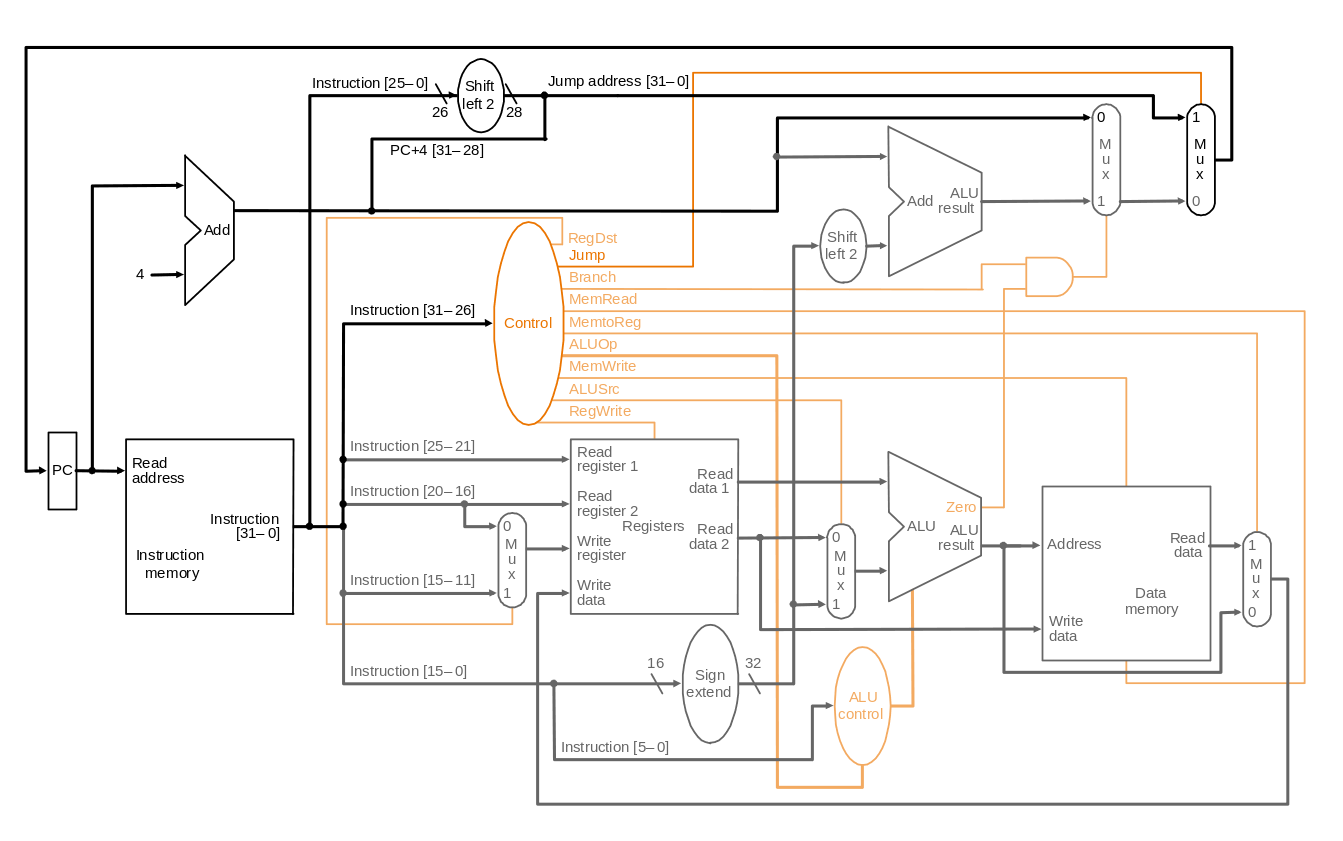
\includegraphics[scale=0.3]{img/single-cycle-cpu.png}
        \caption{Single-cycle CPU with jump and branch.}
        \label{img:single-cycle-cpu}
    \end{figure}
\end{theorem}
